%%%%%%%%%%%%%%%%%%%%%%%%%%%%%%%%%%%%%%%%%%%%%%%%%%%
%% LaTeX book template                           %%
%% Author:  Amber Jain (http://amberj.devio.us/) %%
%% License: ISC license                          %%
%%%%%%%%%%%%%%%%%%%%%%%%%%%%%%%%%%%%%%%%%%%%%%%%%%%

\documentclass[a4paper,10pt]{article}
\usepackage[margin=1.0in]{geometry}
\usepackage[T1]{fontenc}
\usepackage[utf8]{inputenc}
\usepackage{paracol}
\usepackage{lmodern}
\usepackage{amsfonts}
\usepackage{multicol}
\usepackage{hyperref}
\usepackage{graphicx}
\usepackage[english]{babel}
\usepackage{microtype} 
\usepackage[justification=centering, margin=0cm]{caption}  % centers captions automatically
%\usepackage{subcaption}

\usepackage{titlesec}
\renewcommand{\thesection}{}% Remove section references...
\renewcommand{\thesubsection}{\arabic{subsection}}%... from subsections

\usepackage[version=3]{mhchem}
\usepackage{amsmath}
\usepackage{mathtools}
\usepackage[absolute,overlay]{textpos}
\usepackage{graphicx}
\usepackage{bm}
\usepackage[normalem]{ulem}
\usepackage{cancel}
\usepackage{relsize}
\usepackage{enumitem}
\usepackage{pgfpages}
\usepackage{gensymb}
\usepackage{floatrow}  % centers images automatically
\usepackage[authoryear]{natbib} 
\bibliographystyle{plainnat}

\definecolor{ForestGreen}{rgb}{0.13, 0.55, 0.13}


\newcommand\norm[1]{\left\lVert#1\right\rVert}
\newcommand\red[1]{\textcolor{red}{\textbf{#1}}}
\newcommand\blue[1]{\textcolor{blue}{\textbf{#1}}}
\newcommand\yellow[1]{\textcolor{yellow}{\textbf{#1}}}
\newcommand\green[1]{\textcolor{ForestGreen}{\textbf{#1}}}
\newcommand\ds[1]{\displaystyle{#1}}
\renewcommand\b[1]{\textbf{#1}}
\DeclarePairedDelimiterX{\ip}[2]{\langle}{\rangle}{#1, #2}
\DeclareMathOperator*{\argmax}{arg\,max}


\setcounter{tocdepth}{3}
\newcommand{\HRule}{\rule{\linewidth}{0.5mm}}
\setlength{\parindent}{0pt}
\setlength{\parskip}{0.5em}  % paragraph margin
%\setlength{\parskip}{2ex plus 0.5ex minus 0.2ex}

\captionsetup[figure]{font=small,labelfont=small}
\setlist[itemize]{noitemsep, nolistsep, topsep=2pt}
\setlist[enumerate]{noitemsep, nolistsep, topsep=2pt}
\setlength\parindent{0pt}
%\setlength{\belowcaptionskip}{-20pt}
\setlength{\textfloatsep}{2pt}




	% Book's title and subtitle
	\title{\huge \textsc{{Report for the project of the course}} \\
		\huge \textsc{Probabilistic Graphical Models} \\ \ \\ \ \\ \ \\ \ \\ \ \\ \ \\ \ \\
		\Large \textsc{\textbf{Joint Training of a Convolutional Network and a Graphical Model for Human Pose Estimation}}
		\\ \ \\ \ \\ \ \\ \ \\ \ \\ \ \\ \ \\
	}
	% Author
	\author{\Large \textsc{Yue Fan (2564216), Maksym Andriushchenko (2565540)}}
	


\begin{document}
	\maketitle
	\thispagestyle{empty}
	\newpage
	\setcounter{page}{1}
	
\section{1. Introduction and Problem Description}
	We address the problem of single person pose estimation from 2D images. Our method is based on the paper "Joint Training of a Convolutional Network and a Graphical Model for Human Pose Estimation" \cite{cnn_pgm_for_hpe}. A part detector (a Convolutional Neural Network) is used to generate likelihood map or suggestions regarding the positions of body parts. Afterwards, these suggestions are refined by the use of a spatial model (which is implemented as a subnetwork inspired by a Markov random field) to enforce kinematic constraints between body parts. The main contribution of \cite{cnn_pgm_for_hpe} is that the part detector and the spatial model can be trained jointly.
		
	We performed all experiments on Frames Labeled In Cinema (FLIC) dataset introduced in \cite{modec}, which consists of 3987 training images, 1016 testing images of 720x480 resolution. Each image was annotated with the coordinates of the following joints: left/right wrist, left/right elbow, left/right shoulder, left/right hip, left/right eye, and nose. In our experiments, we used all joints except left/right eyes, since we were not interested in such precise localization, and decided that the position of a nose is enough.
	
	Our own contribution goes as follows: 
	\begin{enumerate}
		\item We reproduced the results of \cite{cnn_pgm_for_hpe}, considerably improving the part detector (without changing its architecture).
		\item We show how to train the model jointly from the beginning, opposed to the proposed 3-staged approach to train the part detector and the spatial model separately and only then do joint training.
		\item We show how to train the joint model much faster: 10 hours instead of 60 hours described in \cite{cnn_pgm_for_hpe}.
		\item Unlike \cite{cnn_pgm_for_hpe}, we explain and show what kind of spatial relations the spatial model has learned.
	\end{enumerate}




\section{2. Approach}
	\subsection{Architecture of the Part Detector}
	The authors proposed to use a Convolutional Neural Network (CNN) for a detector of joints positions. They describe a series of architectures, but we will focus only on the last one, which was implemented used in the paper (see Fig. \ref{cnn_architecture}).
	\begin{figure}[H]
 		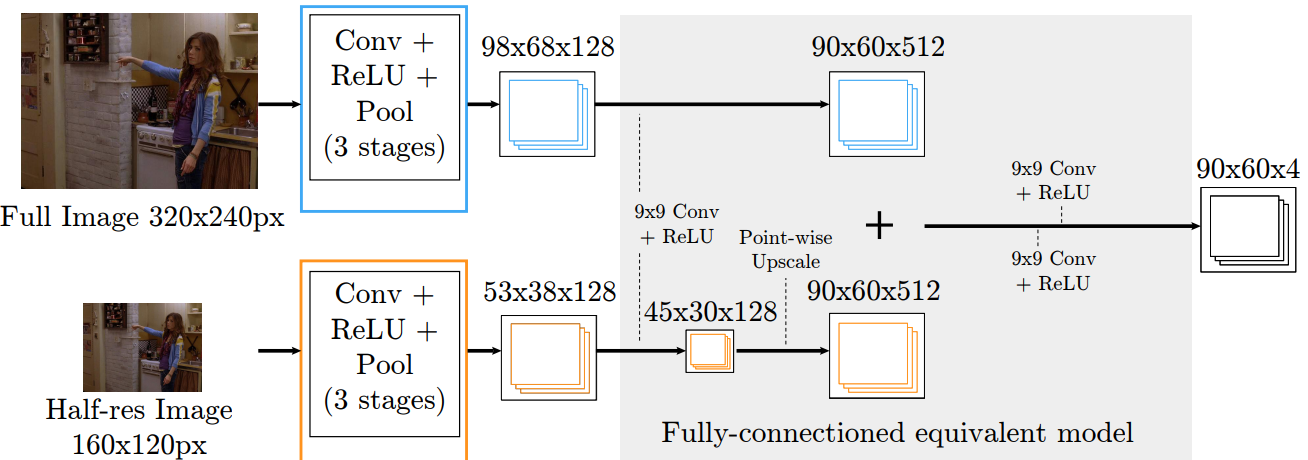
\includegraphics[height=4.5cm]{img/cnn_architecture.png}
		\caption{CNN architecture. Source: \cite{cnn_pgm_for_hpe}.}
		\label{cnn_architecture}
	\end{figure}
	First of all, they propose a fully-convolutional approach. As input they use multiple images of different resolutions that aim to capture the spatial context of a different size. These images are processed by a series of 5x5 convolutional and max pooling layers. Then the feature maps from different resolutions are added up, followed by 2 large 9x9 convolutions. The final layer with 90x60xK feature maps (where K is the number of joints) is our predicted heat maps. We use then softmax and cross-entropy loss on top of them together with the ground truth heat maps, which we form by placing a small 3x3 binomial kernel on the actual joint position. 
	
	Note, that the input resolution 320x240 is not justified at all in the paper, and it is not clear how one can arrive at 98x68 or 90x60 feature maps after 2 max pooling layers. We consider this as a mistake, and instead use what makes more sense to us: processing of the full resolution 720x480 images, but the first convolution is applied with stride=2, making all dimensions of feature maps comparable in size with what proposed in the paper.
	
	The described part detector already gives good results (see first two images on Fig. \ref{our_pd_examples}), however, there are also some mistakes that potentially can be ruled out by applying a spatial model. For example, in the third image of Fig. \ref{our_pd_examples} there are many false detections of hips (pink color), which clearly do not meet kinematic constraints w.r.t. nose and shoulders that are often detected with very high accuracy.
	\begin{figure}[H]
		\begin{tabular}{ccc}
			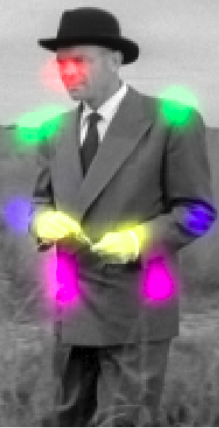
\includegraphics[height=5cm]{img/ex1.png} & 
			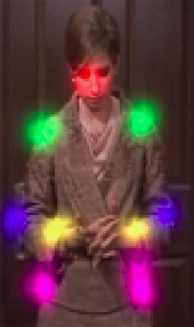
\includegraphics[height=5cm]{img/ex2.png} &
			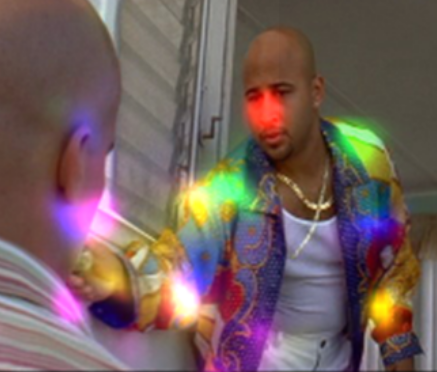
\includegraphics[height=5cm]{img/ex3.png} 
			\caption{The examples from \textit{our part detector} (without spatial model). We will use the following color scheme throughout the report: red - nose, green - shoulders, blue - elbows, yellow - wrists, pink - hips. }
			\label{our_pd_examples}
		\end{tabular}
	\end{figure}


	\subsection{Architecture of the Spatial Model}
	So our goal is to get rid of such false positives that clearly do not meet kinematic constraints. Traditionally, for such purposes a probabilistic graphical model was used. One of the most popular choices is tree-structured graphical models (\cite{andriluka2009pictorial}, \cite{pishchulin2013strong}, \cite{pishchulin2013poselet}). The inference is exact in these models and also efficient due to gaussian pairwise priors which are most often used. Some approaches combined exact inference with a hierarchical structure of a graphical model (\cite{tian2012exploring}). Another approaches relied on approximate inference with a loopy graphical model (\cite{lan2005beyond}, \cite{karlinsky2012using}), that allowed establishing connections between symmetrical parts.
	
	An important novelty of \cite{cnn_pgm_for_hpe} is that the spatial model can be modeled as a fully connected graphical model with parameters that can be trained jointly with the part detector. Thus the graphical model can be learned from the data, and there is no need to design it for a specific task and dataset, which is a clear advantage. They propose to calculate the marginal likelihood of joint location $\bar{p}_A$ as:
	\begin{equation*}
		\bar{p}_A = \frac{1}{Z} \prod_{v \in V} (p_{A|v} * p_v + b_{v \rightarrow A})
	\end{equation*}
	where $p_v$ is the likelihood map obtained by the part detector, $p_{A|v}$ is the conditional prior that is learned with backpropagation, $V$ is the set of all joints except $A$, $b_{v \rightarrow A}$ is a bias or background probability for the message $v \rightarrow A$, Z is the partition function, and * denotes convolution. The authors claim that it can be seen as a single round of sum-product belief propagation in a loopy fully-connected graphical model. So this approach provides only an approximate inference in a graphical model, however, the authors claim that it is still sufficiently accurate in order to capture the main kinematic constraints of the human body.
	
	The final expression includes energies instead of probabilities and they evaluate it in the log-space because it considerably simplifies taking derivatives w.r.t. parameters:	
	\begin{equation*}
		\bar{p}_A = \frac{1}{Z} exp \left(  \sum_{v \in V}  log \Big( s(e_{A|v}) * s(e_v) + s(b_{v \rightarrow A})  \Big) \right)
	\end{equation*}
	where $e_v$ is the likelihood energy obtained by the part detector, $e_{A|v}$ is the conditional energy parameter matrix between two joints (learned with backpropagation), and $s(x) = \frac{1}{\beta} log(1 + exp(\beta x)$ (we used $\beta = 5$). Note that authors use ReLU instead of second softplus, but do not motivate their choice. We found that using softplus everywhere leads to a similar performance, especially given that softplus can be seen as a differentiable approximation of ReLU, so we decided to keep it consistent and use softplus everywhere. Its main goal is to maintain energies strictly positive, which softplus does. Also note that the partition function $Z$ is skipped in the paper. However, we evaluate it, since cross-entropy loss is well-motivated only if we have probabilities. So the final objective of the spatial model is to minimize cross-entropy loss between marginal probabilities of joints and target heat maps.
	
	On Fig. \ref{example_pd_vs_sm} we can see a few examples of how our spatial model trained jointly with the part detector performs compared to the part detector only.
	\begin{figure}[H]
		\begin{tabular}{ccc}
			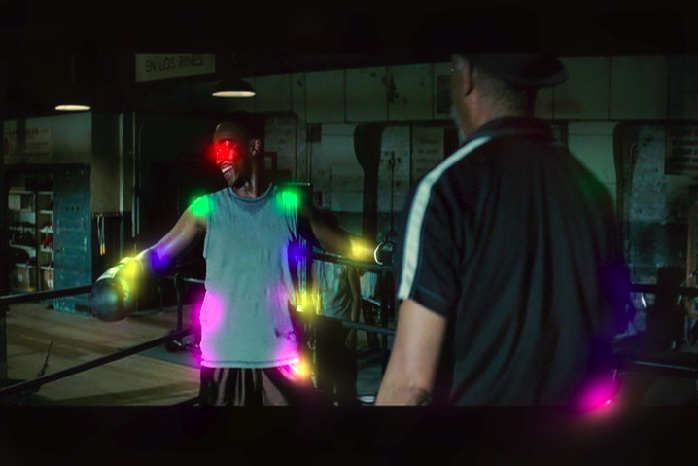
\includegraphics[height=4cm]{img/pd1.png} & 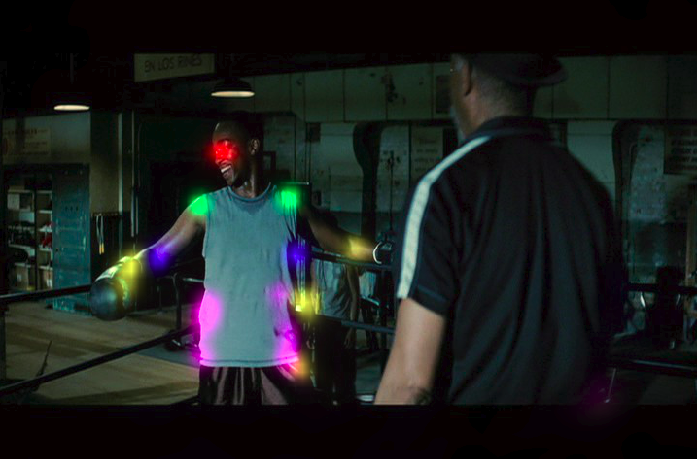
\includegraphics[height=4cm]{img/sm1.png} \\
			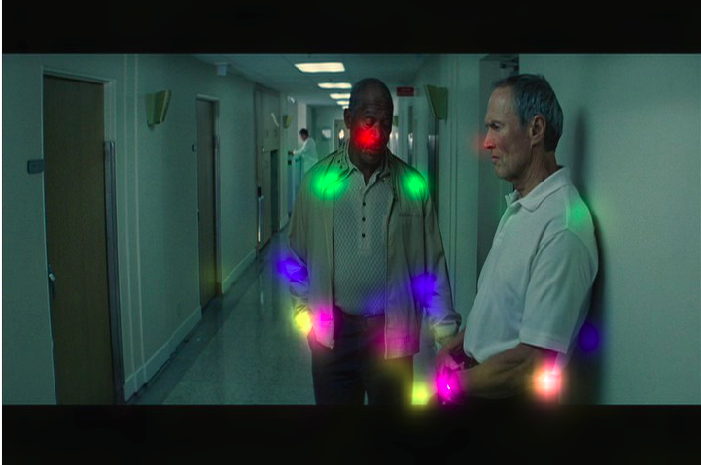
\includegraphics[height=4cm]{img/pd2.png} & 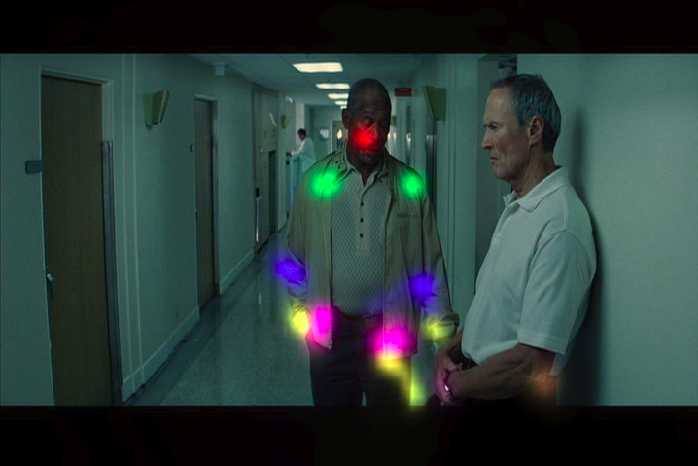
\includegraphics[height=4cm]{img/sm2.png} 
			\caption{Left column: part detector. Right column: part detector and spatial model.}
			\label{example_pd_vs_sm}
		\end{tabular}
	\end{figure}
	On the 1st example we can see that there is a detection of hip of backward facing person. However, this hip does not have any other body parts in its vicinity, so it is ruled out by the spatial model.
	On the 2nd example there are a few joint detections of the person standing on the right, and also a minor detection of a wrist on the left (small yellow cloud). All of them are ruled out by the spatial model. Note, that there are still some mistakes, but rigorous model evaluation in Section~3 reveals that we indeed get a significant improvement by applying the spatial model.
		
	
	\subsection{Our Improvements}
	\begin{enumerate}
		\item We train the model 6 times faster by using Batch Normalization (\cite{ioffe2015batch}), inserted after each activation function (as recommended by \cite{mishkin2017systematic}), and cross-entropy loss instead of the squared loss. Apart from faster training we also achieved better test loss and test detection rate.
		\item We use an auxiliary classifier on heat maps generated by the part detector. This approach is inspired by \cite{girshick2015fast} and \cite{conv_pose_machines}. The idea is to make \textit{both} the part detector and the spatial model to output reasonable heat maps, not only the spatial model. We found this to improve the results.
		\item We used Adam from \cite{adam} in order to perform joint training for both part detector and spatial model with a single set of optimizer's hyperparameters. We tried to use SGD with Momentum as suggested in \cite{cnn_pgm_for_hpe}, but the spatial model requires completely different learning rate and potentially different momentum coefficient. Thus we decided to stick to Adam, which is known to work very well for different functions with the default parameters. Finally, we trained the joint model for 60 epochs with the initial learning rate divided by 2, 5, and 10 after 70\%, 80\%, and 90\% epochs.
		\item As was mentioned above, we use the whole input images without any special preprocessing. Since the initial image resolution (720x480) is quite big, we apply the first convolution with stride 2. In this way we don't discard any information from the dataset (as opposed to 320x240 crop mentioned in the diagram of the CNN, but not explained further in the text).	
		\item We use more advanced data augmentation scheme including horizontal mirroring (with probability 50\%), random change of contrast and brightness, random rotation (from -10$\degree$ to +10$\degree$), and random cropping.
		\item We applied the weight decay only to convolutional filters in the part detector, but not to the spatial model. Because we observed that the highest absolute values of pairwise potentials and biases are quite moderate, and biasing the potentials towards zero is not well motivated.	
		\item We excluded self-connections like face$\rightarrow$face from the spatial model, which did not make much sense to use and which did not contribute to the final performance.
	\end{enumerate}
	Combining all details mentioned above we improved the final results compared to \cite{cnn_pgm_for_hpe}. We also did not observe any benefit in terms of the test detection rate using three-staged training procedure described in the paper. Thus we adopt joint end-to-end training of both the part detector and the spatial model from the very beginning. All results shown in Section 3 correspond to this approach. Finally, we provide more examples of our model's joint detections in the appendix (see Fig. \ref{appendix} and Fig. \ref{appendix_evolution}).
	

	\subsection{Reproducibility Challenge}
	The paper \cite{cnn_pgm_for_hpe} was extremely hard to reproduce. Here are a few reasons why:
	\begin{itemize}
		\item The original code of the model was not published.
		\item The hyperparameters and random initialization scheme are not mentioned. Since originally they had 3 stages of training, we assume that such procedure may need 3 sets of hyperparameters. Most importantly, we were curious about the learning rates and the number of epochs to train the models on each stage.
		\item We had to adopt the multi-scale evaluation procedure from \cite{prev_iclr_paper}. This alone gives around +6\% detection rate for wrists. We are quite sure that it was used in \cite{cnn_pgm_for_hpe}, however there are \textit{no mentions of this procedure}. Without this we could not match the performance of their part detector.
		\item \cite{prev_iclr_paper} also mentions quite complicated preprocessing of FLIC training images, which includes manual annotation of the bounding box of the head, and which aims to crop the images in a way that all humans are on the same scale. We tried to apply a procedure similar to this, but it did not lead to successful results. We still think that there was some preprocessing step that could potentially lead to even better results than in our implementation.
		\item For evaluation and training they flipped left and right joints of backward facing people. We found this only by inspecting their evaluation code available at \url{https://cims.nyu.edu/~tompson/data/flic_lsp_predictions.zip}.
		\item They do not show the detection rate for all joints, but only for wrist and elbow. They chose to show left wrist/elbow, simply because they give better results than right wrist/elbow, and they did not mention this. However, we observed quite a significant gap between left and right wrists with single-scale evaluation scheme. However, with multi-scale evaluation, the difference is minor.
	\end{itemize}
	This explains why we could not find any implementation of this paper on the internet. Therefore our TensorFlow implementation \url{https://github.com/max-andr/joint-cnn-mrf} is the first one, which hopefully can be useful for some research or didactic purposes.
	
	
	
	
	
\section{3. Results}	

	\subsection{Evaluation}
	
	We used the same evaluation metric as \cite{cnn_pgm_for_hpe}, which was first proposed in \cite{modec}:
	\begin{equation*}
		acc_i(r) = \frac{100}{N} \cdot \sum_{t=1}^{N} \textbf{1} \left( \frac{100 \cdot ||y_i^{t'} - y_i^{t}||_2}{||y_{lhip}^{t} - y_{rsho}^{t}||_2} \right)
	\end{equation*}
	where $i$ is the particular joint, $r$ is the detection radius, $N$ is the test size, $y_i^{t'}$ is the predicted coordinates of the joint $i$ of the test example $t$, $y_i^{t}$ is the true coordinates of the joint $i$ of the test example $t$. We will refer to this metric as \textit{detection rate} or simply \textit{accuracy}. Its main idea is to measure the joint localization inside some radius expressed in pixels normalized by the torso size. 

	The evaluation of our model is presented on Fig. \ref{our_detrate} and the results from the original paper are on Fig. \ref{orig_detrate}.
	\begin{figure}[H]
		\begin{tabular}{cc}
			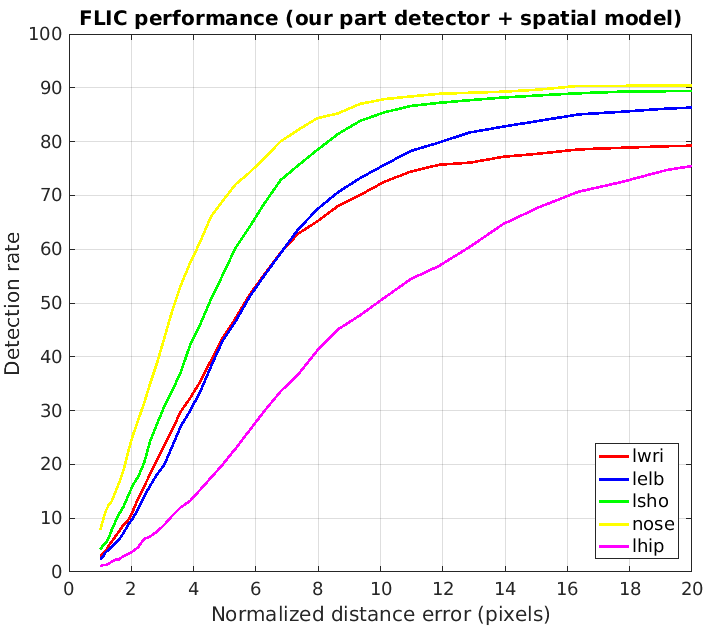
\includegraphics[height=5cm]{img/our_pd_detrate.png} & 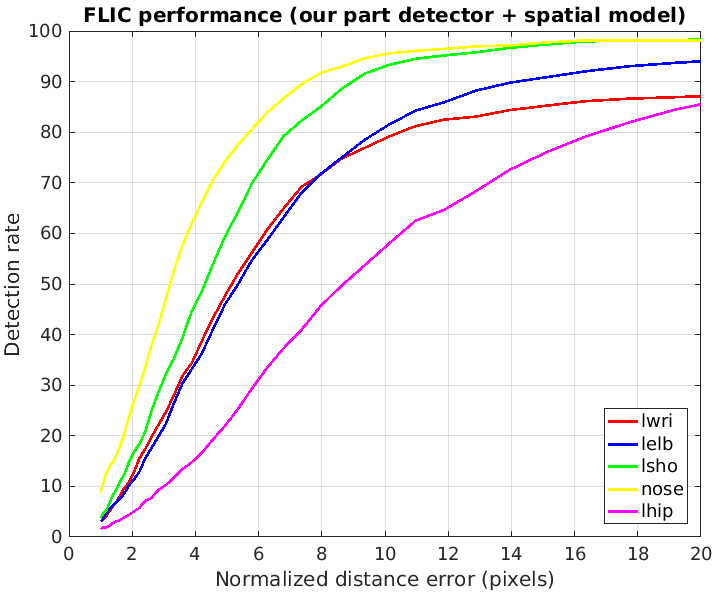
\includegraphics[height=5cm]{img/our_pdsm_detrate.png} 
			\caption{The accuracy of \textit{our model} without (left) and with spatial model (right).}
			\label{our_detrate}
		\end{tabular}
	\end{figure}
	\begin{figure}[H]
		\begin{tabular}{cc}
			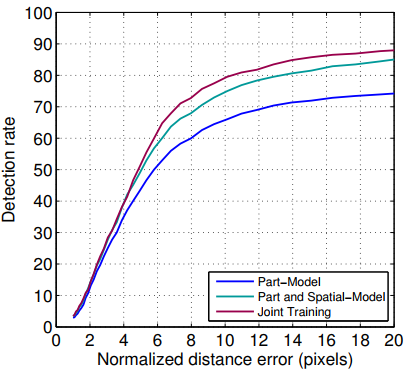
\includegraphics[height=5cm]{img/orig_wrist_detrate.png} &
			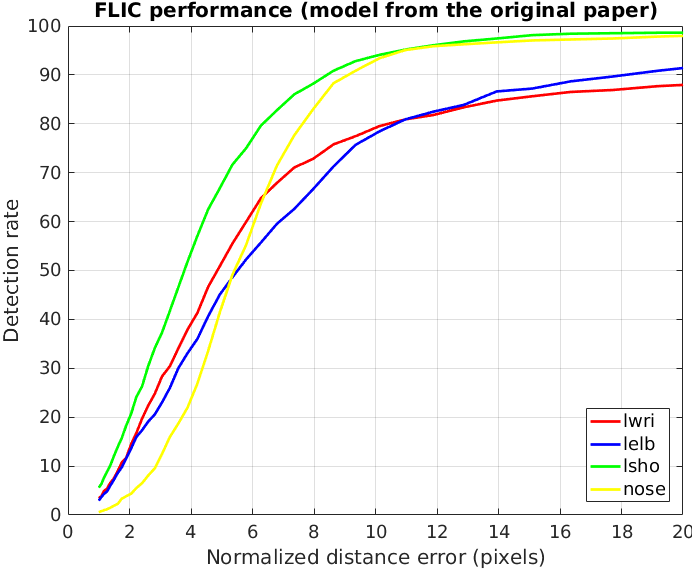
\includegraphics[height=5cm]{img/orig_pdsm_detrate.png} 
			\caption{The accuracy of the \textit{original model}. Note, that they did not provide results for hips in their files. Source: \cite{cnn_pgm_for_hpe}, \url{https://cims.nyu.edu/~tompson/data/flic_lsp_predictions.zip}.}
			\label{orig_detrate}
		\end{tabular}
	\end{figure}
	Let's consider radius of 10 normalized pixels for the analysis. We can observe that our part detector gives +6\% accuracy for the left wrist (Fig. \ref{our_detrate}, plot 1) compared to the original part detector (Fig. \ref{orig_detrate}, plot 1). After applying the spatial model, our model (Fig. \ref{our_detrate}, plot 2) has \textbf{the same accuracy for the left wrist and left shoulder} (compared to Fig. \ref{orig_detrate}, plot 2). However, \textbf{our model has 3\% better accuracy for left elbow and for the nose}. 
	
	Interestingly, if we consider the accuracy with low radius, our model has much better accuracy for the nose, while the original model has much better accuracy for left shoulder. In our opinion, the choice of the loss function and the way one models probabilities (element-wise sigmoid or softmax over a heat map) has the crucial role here.
	
	
	\subsection{Analysis of Spatial Model}
	
	We note that the original paper completely skipped the part what their spatial model actually learned. However, the most interesting question is what kind of parameters for pairwise potentials were learned with backpropagation. We show them on Fig. \ref{pairwise_pots}. Please, note that we show pre-softplus values, but after softplus values are obviously similar except negative values.
	\begin{figure}[H]
		\begin{tabular}{ccc}
			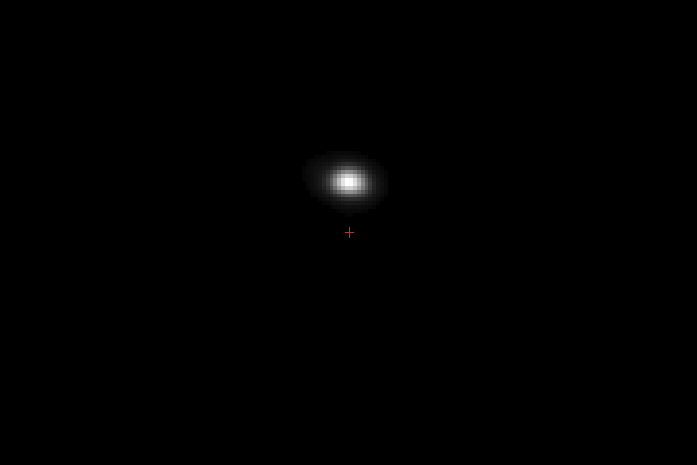
\includegraphics[height=2.8cm]{img/0epoch_nose_torso.png} & 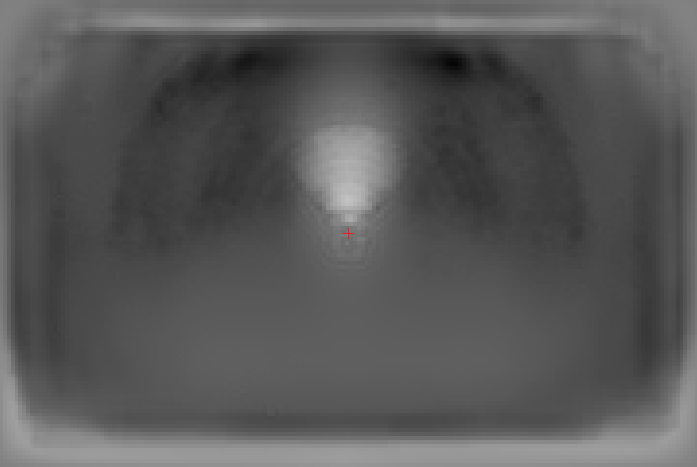
\includegraphics[height=2.8cm]{img/60epoch_nose_torso.png} & 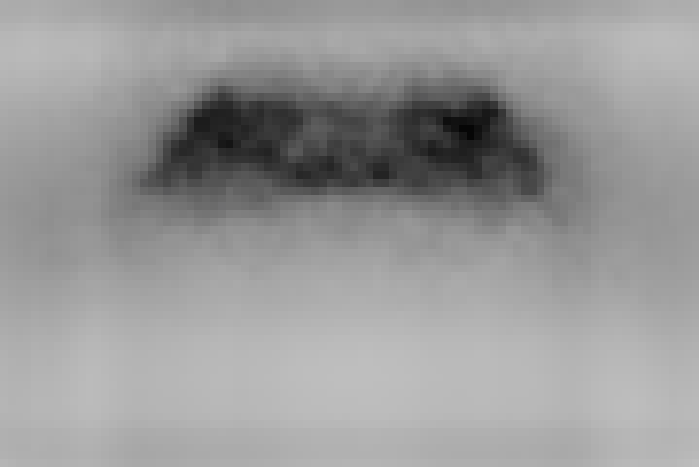
\includegraphics[height=2.8cm]{img/60epoch_bias_nose_torso.png} \\
			initial $e_{nose | torso}$ & $e_{nose | torso}$ after 60 epochs & $b_{torso \rightarrow nose}$ after 60 epochs \\
			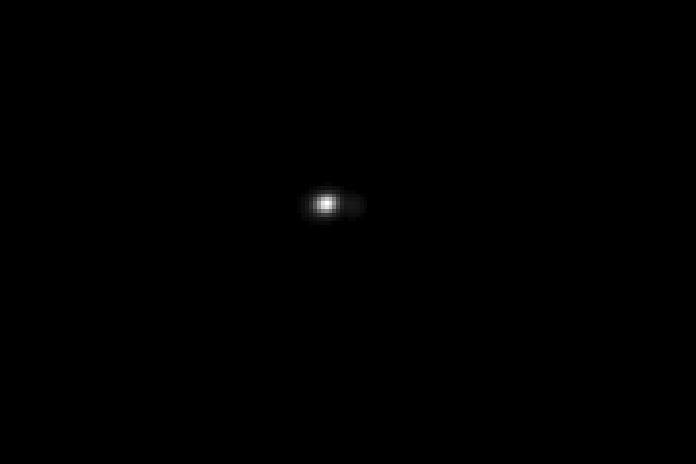
\includegraphics[height=2.8cm]{img/0epoch_rsho_torso.png} & 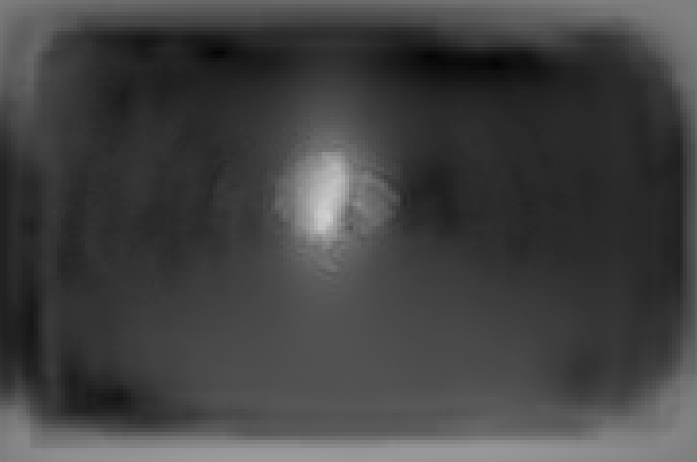
\includegraphics[height=2.8cm]{img/60epoch_rsho_torso.png} & 
			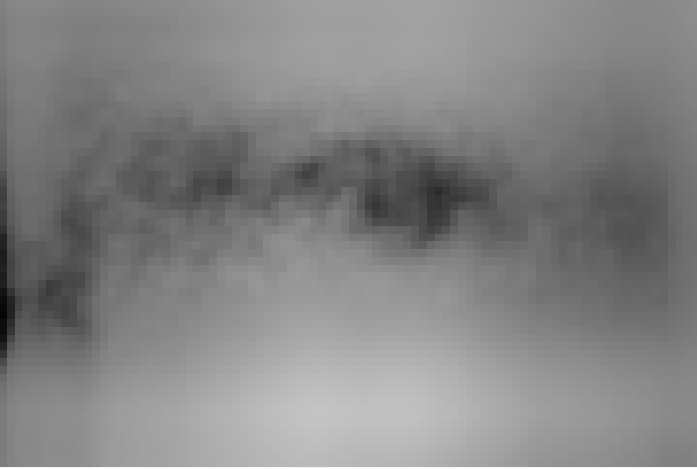
\includegraphics[height=2.8cm]{img/60epoch_bias_rsho_torso.png}\\
			initial $e_{rsho | torso}$ & $e_{rsho | torso}$ after 60 epochs & $b_{torso \rightarrow rsho}$ after 60 epochs \\
			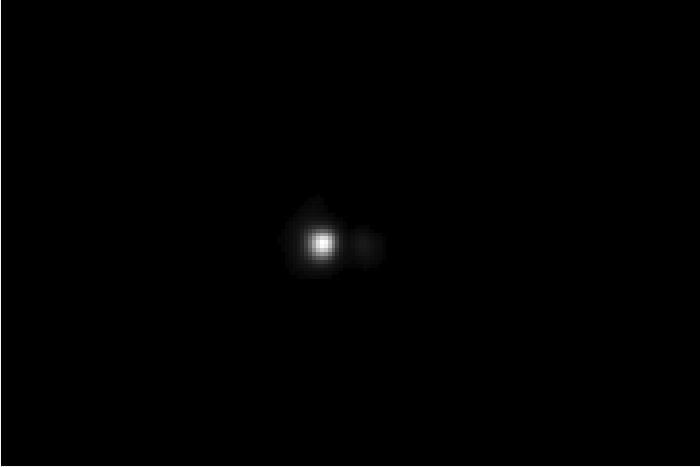
\includegraphics[height=2.8cm]{img/0epoch_relb_torso.png} &
			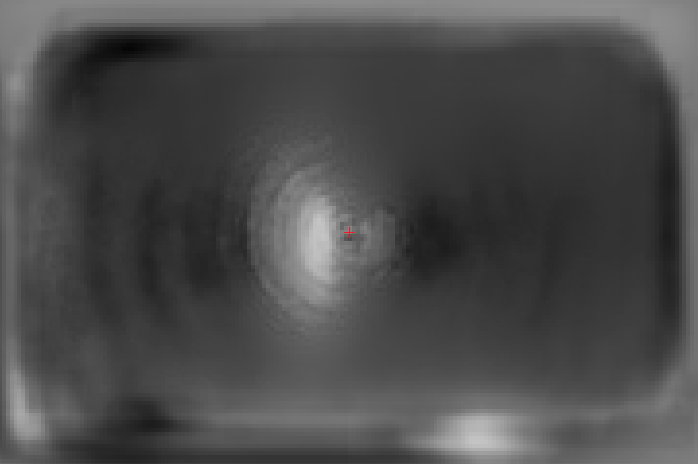
\includegraphics[height=2.8cm]{img/60epoch_relb_torso.png} & 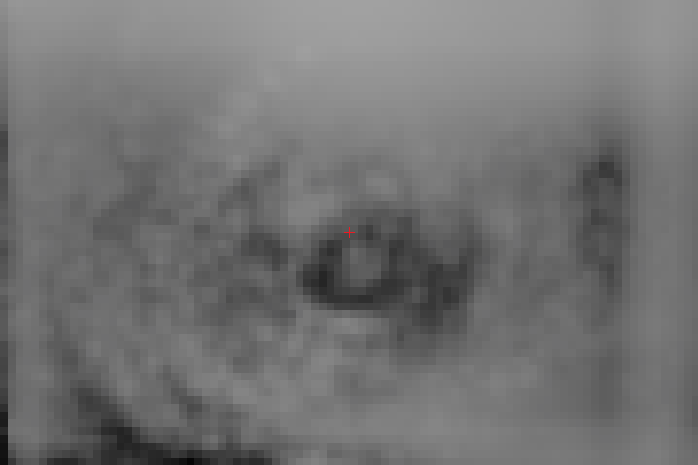
\includegraphics[height=2.8cm]{img/60epoch_bias_relb_torso.png} \\
			initial $e_{relb | torso}$ & $e_{relb | torso}$ after 60 epochs & $b_{torso \rightarrow relb}$ after 60 epochs
			\caption{Visualization of parameters corresponding to potentials learned in \textit{our spatial model}. First col.: initialized parameters based on empirical histogram of joint displacements. Second col.: parameters after 60 epochs. Third col.: pairwise biases after 60 epochs. \\
			White color denotes high values of parameteres, and dark denotes low values.}
			\label{pairwise_pots}
		\end{tabular}
	\end{figure}
	
	We show only potentials of joints conditioned on the torso (Fig. \ref{pairwise_pots}) because this leads to more distinct patterns. In contrast, $e_{lhip | rwri}$ has almost uniform distribution, which means that this connection in a graphical model is redundant. 
	
	We can notice that for nose and right shoulder we have a much more concentrated picture than for right elbow since there is less ambiguity on where this part can appear relative to the center of the torso. Also note the circular patterns, especially on $e_{relb | torso}$, which are there because of the usage of rotated images (from -10$\degree$ to 10$\degree$) in data augmentation. We can also observe that during training all pairwise parameters have changed a lot comparing to the initialization (first column). The borders have grey frames because these values were not actually trained since border values represent energies for very high displacements of locations between two joints, which are not encountered in the training dataset. So they stayed zeros as they were initialized in the beginning.
	
	The interpretation of bias terms is rather unclear. Authors claim that their purpose is to correct false negatives produced by the part detector. We cannot confirm this idea by observing from Fig. \ref{pairwise_pots}.
	
    
    
    
    \section{4. Conclusions}
    The approach proposed in this paper is \textit{conceptually interesting} since it allows to perform a joint training of a convolutional neural network and a graphical model, which is implemented as a separate subnetwork that uses the output of the CNN. We further simplified the proposed training procedure to a single stage of joint training and showed how to make the training 6 times faster. However, the graphical model in the paper has one disadvantage: it is not scale-invariant, which explains a strong need for multi-scale evaluation.
    
    This approach has led to the state-of-the-art performance as for 2014. Although the most important advance of the paper is actually the part detector that operates on images of different resolution, which is even without the graphical model part achieved state-of-the-art results. The graphical model part has obviously increased the margin even further. 
    
    However, it seems that very recent advances in CNNs allow to completely skip a graphical model part of the pipeline in human pose estimation task. In other words, CNN itself can learn the main kinematic constraints, given that it has big enough receptive field and enough data. \cite{conv_pose_machines} shows the importance of the receptive field size (see Fig. \ref{rec_field}) and significantly outperforms the results of \cite{cnn_pgm_for_hpe} without any graphical model.
    
    \begin{figure}[H]
    	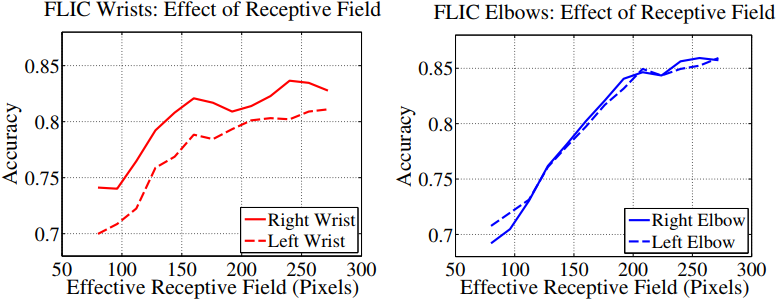
\includegraphics[height=4cm]{img/receptive_field_importance.png}
    	\caption{Importance of receptive field size. Source: \cite{conv_pose_machines}}
    	\label{rec_field}
    \end{figure}
    This also means that using novel CNN architectures like VGG (\cite{vgg}) or ResNets (\cite{resnets}) as a part detector can improve the performance considerably (e.g. see the results of \cite{deepcut}, \cite{deepercut}, but note that their GraphCut approach leads to significant improvements only for a multi-person pose estimation task). This can be explained by the huge receptive fields of these extremely deep networks, so they do not even require a graphical model on top of them since they already can learn relations between the body parts. However, graphical models seem to play an important role in other tasks, especially when the training data is scarce.
    
    
 
 
	\newpage
	\renewcommand{\thepage}{}
	\bibliographystyle{apalike}
	\bibliography{references}
	\newpage
	
	
	\section{Appendix}
	Here are more examples of our final model (Fig. \ref{appendix}) without any hand selection. Note, that softmax may be not very suitable for multi-person human pose estimation as was mentioned in \cite{deepcut}, because in that case, we may need to assign very high probabilities ($\approx$ 1) to the same joints of different people. However, in FLIC dataset only one person is annotated on each image, so for this particular dataset softmax is a reasonable choice.
	\begin{figure}[H]
		\begin{tabular}{cc}
			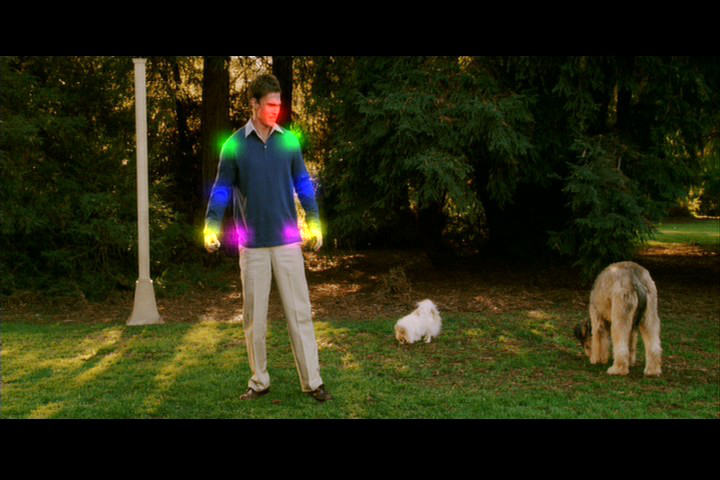
\includegraphics[height=4.9cm]{img/ap_sm1.png} & 
			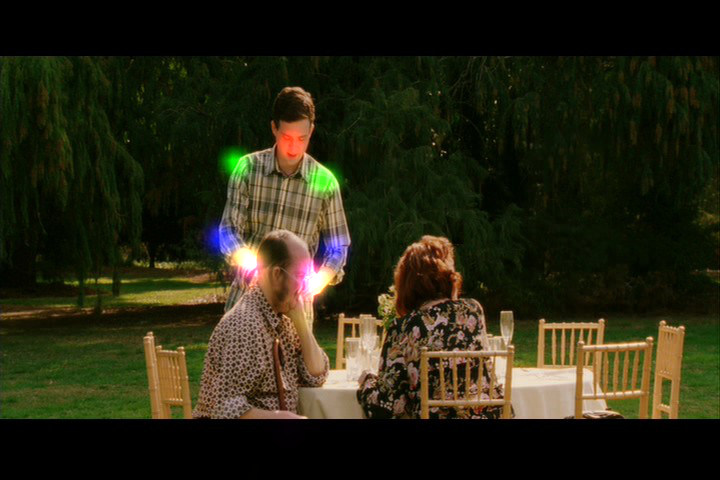
\includegraphics[height=4.9cm]{img/ap_sm2.png} \\
			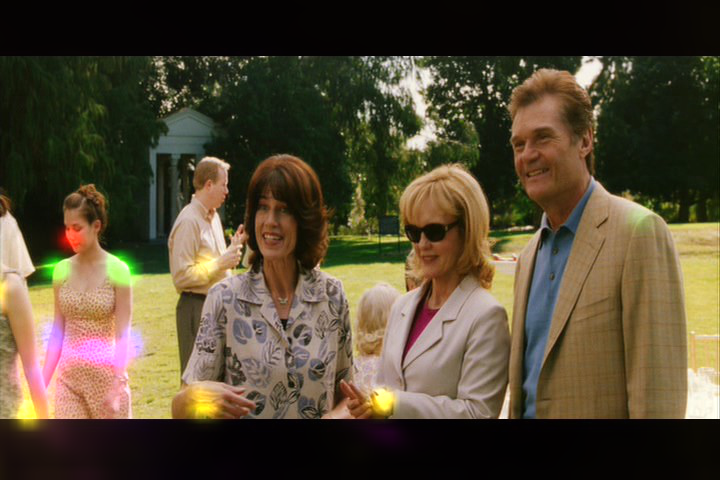
\includegraphics[height=4.9cm]{img/ap_sm3.png} &
			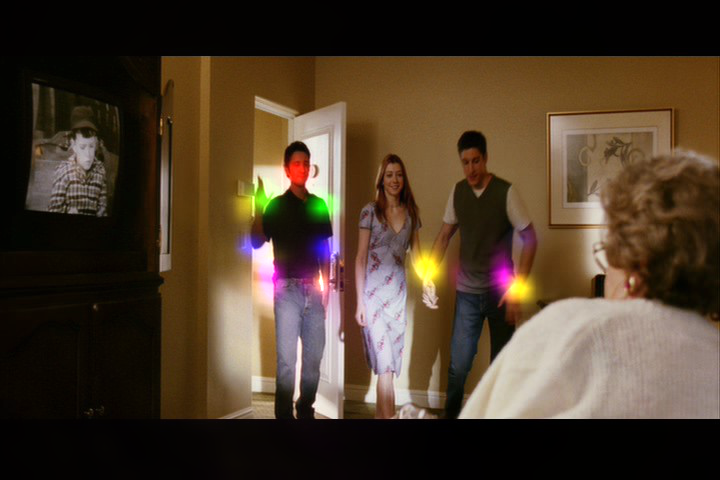
\includegraphics[height=4.9cm]{img/ap_sm4.png} \\
			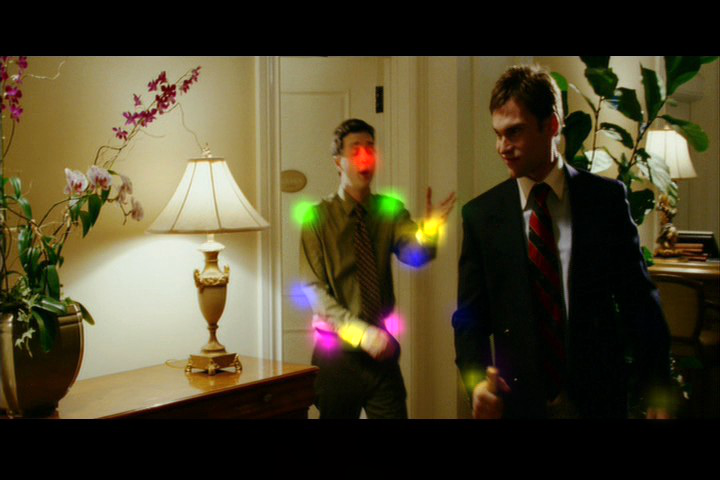
\includegraphics[height=4.9cm]{img/ap_sm5.png} & 
			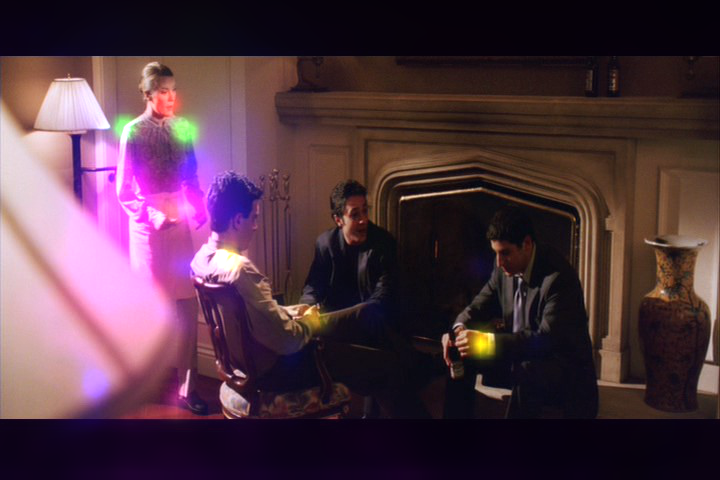
\includegraphics[height=4.9cm]{img/ap_sm6.png} \\
			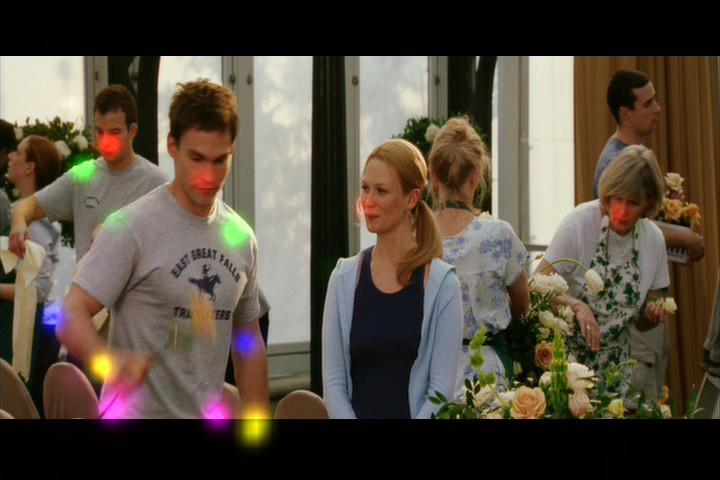
\includegraphics[height=4.9cm]{img/ap_sm7.png} &
			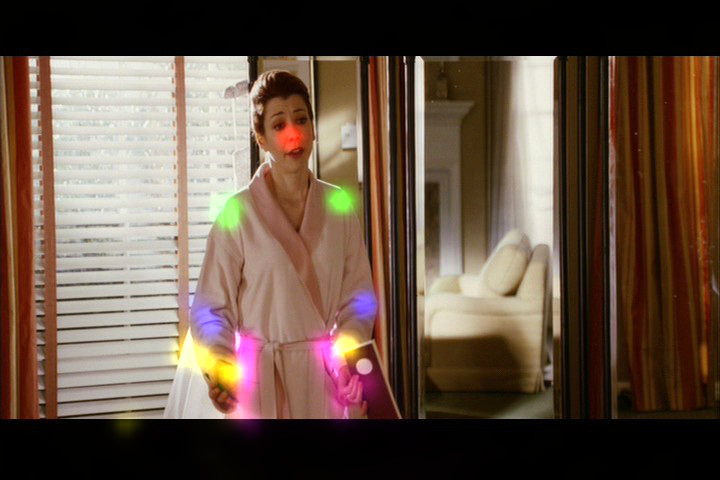
\includegraphics[height=4.9cm]{img/ap_sm8.png}
			\caption{More examples from \textit{our model} (part detector + spatial model together)}
			\label{appendix}
		\end{tabular}
	\end{figure}
	
	\newpage	
	And also we show in Fig. \ref{appendix_evolution} how the model improves its performance over training (3, 20, 40 and 60 epochs respectively). Note, that even after 3 iterations nose and shoulders are almost perfectly localized, which reveals the fact that not all joints are equally hard to detect.
	\begin{figure}[H]
		\begin{tabular}{cc}
			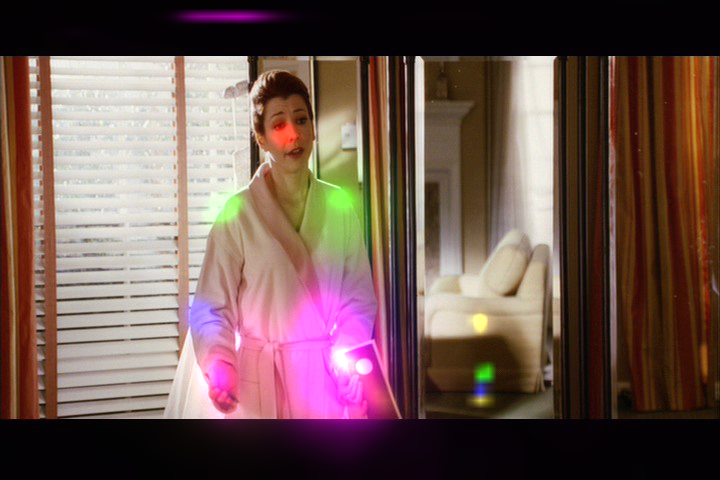
\includegraphics[height=5cm]{img/ap_epoch3.png} & 
			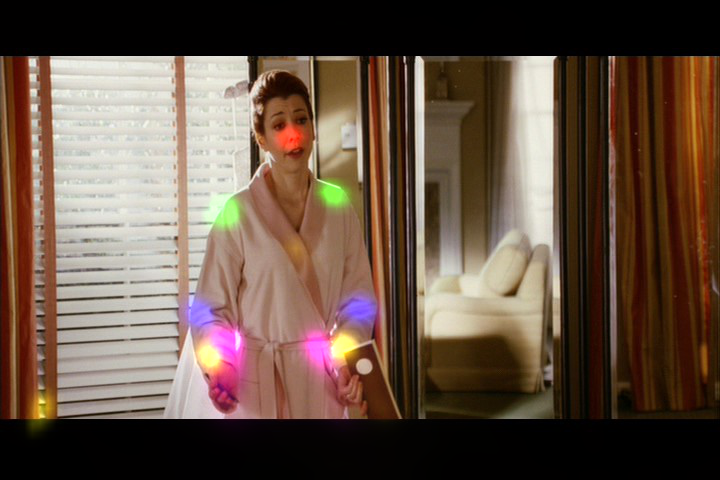
\includegraphics[height=5cm]{img/ap_epoch20.png} \\
			Joints detection after 3 epochs & Joints detection after 20 epochs \\
			& \\
			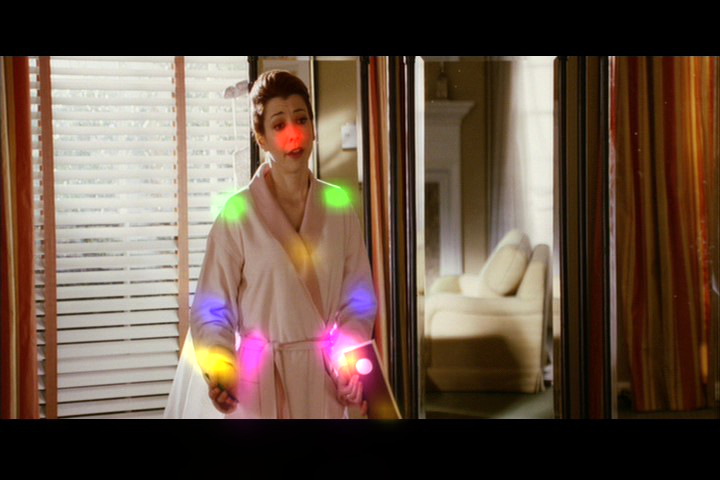
\includegraphics[height=5cm]{img/ap_epoch40.png} &
			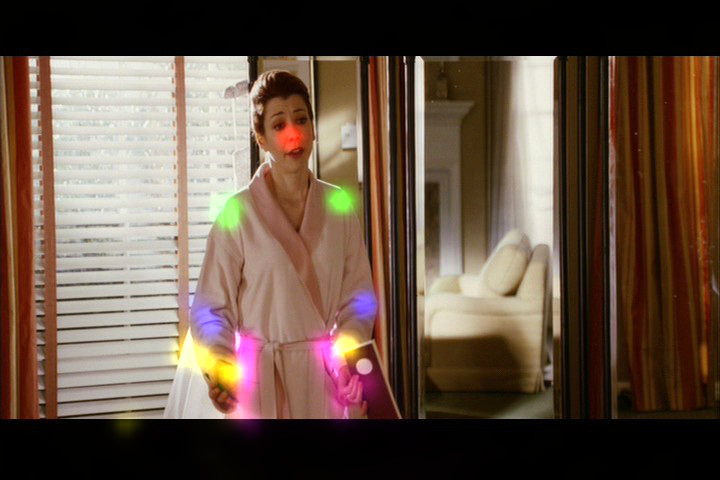
\includegraphics[height=5cm]{img/ap_epoch60.png} \\
			Joints detection after 40 epochs & Joints detection after 60 epochs
			\caption{Improvement of \textit{our model} over training (part detector + spatial model together)}
			\label{appendix_evolution}
		\end{tabular}
	\end{figure}

\end{document}


